%
% TU/e Style Master Thesis template for LaTeX
%
% Public version 1.0
% 2010 - 2013 Thijs Nugteren and Joos Buijs
%
% THIS IS THE MAIN FILE (i.e. compile this file, compiling the others directly won't work)
%
\documentclass[a4paper,10pt,twoside]{report}

%all the other includes etc. are done in the thesis.sty file.
\usepackage{thesis}

% 
% These commands need to be defined in order to produce a correct and personalized document

%
\newcommand{\shortdoctitle}{Benchmark Studies}
\newcommand{\doctitle}{Benchmark Studies of Various Deep Learning Architecture}
\newcommand{\docsubtitle}{Data Mining Seminar}

\newcommand{\me}{Irfan Nur Afif}
\newcommand{\keywords}{keyword1, keyword2, keyword3}
\newcommand{\version}{version 1.0}
\newcommand{\monthYear}{December 2017}

%Be sure to use all the titles for your committee members!!! (their names show up on the very first page!)
\newcommand{\firstCommitteeMember}{Joaquin Vanschoren}
\newcommand{\secondCommitteeMember}{Your second Committee Member, usually the daily supervisor}
\newcommand{\thirdCommitteeMember}{Your Third Committee Member, usually the external member}

\author{\me}

%
% PDF settings
%
\hypersetup
{
    pdfauthor={\me},
    pdftitle={\shortdoctitle},
    pdfsubject={\doctitle},
    pdfkeywords={\keywords}
}

\begin{document}

%use this include for PDF and distribution versions
\pagenumbering{roman}
\begin{titlepage}
\begin{center}

\includegraphics[height=2cm]{figures/tue-logo-high}\\
%\LARGE
%Eindhoven University of Technology \\
\large
Department of Mathematics and Computer Science  \\
Data Mining Research Group

\vspace*{10cm}

\setlength{\TPHorizModule}{1mm}
\setlength{\TPVertModule}{\TPHorizModule}
% Set the Paragraph Indent to zero, so the first line is not Indented
% Back-up the current value so it can be put back at the end of the title page
\newlength{\backupparindent}
\setlength{\backupparindent}{\parindent}
\setlength{\parindent}{0mm}			
% Begins a textbox at 72 mm from the left of the edge of the paper and 89 mm from the top
% The width of the textbox is 95 mm (167 - 72 mm)
% The height of the box cannot be defined, so it is your task to keep the text not too long
\begin{textblock}{95}(62,89)
    \vspace*{1mm}
    \huge
    \textbf{\doctitle \\}
    \Large
    \vspace*{5mm}
    \textit{\docsubtitle}\\
    \vspace*{10mm}
    \Large
    \me\\
\end{textblock}

\large
Supervisors:\\
\begin{tabular}{rl}
    \firstCommitteeMember\\
    %\secondCommitteeMember\\
    %\thirdCommitteeMember\\
\end{tabular}

\vfill
\version

\vfill
%\docdate \\
\large
Eindhoven, \monthYear\\

% Put the Paragraph Indent back to its original value
\setlength{\parindent}{\backupparindent}
\end{center}
\end{titlepage} 

\normalsize

%\clearemptydoublepage

%Sometimes line numbers are nice, uncomment the next line to enable:
%\linenumbers

%It could be handy to have a list of todos and brainstorms in your thesis
%\chapter*{*General todos*}\todo{remove this chapter}
%\input{chapters/general_todos}

%\chapter*{*Brainstorm results*}\todo{remove this chapter}
%\input{chapters/brainstorm_results}

%\chapter*{Abstract}\label{chapter:abstract}
%THIS IS MY ABSTRACT

%\clearemptydoublepage

%An executive summary if you want:
%\chapter*{Executive summary}\label{chapter:executive_summary}
%\input{chapters/executive_summary}

%\clearemptydoublepage


%\chapter*{Preface}\label{chapter:preface}
%Please write all your preface text here. If you do so, don't forget to thank your supervisor, other committee members, your family, colleagues etc.\ etc. 

%\clearemptydoublepage

\tableofcontents

%\clearemptydoublepage

%\listoffigures

%\clearemptydoublepage

%\listoftables

%\clearemptydoublepage

%\lstlistoflistings

%\clearemptydoublepage

\chapter{Introduction}\label{chapter:introduction}
\setcounter{page}{0}
\pagenumbering{arabic}
%from here on, start the 'real' page numbering, from 1, with normal digits
\section{Context \& Motivation}
Machine learning has become an integral part of today's technology. It has a lot of applications in our daily lifes, for example a recommender system or a prediction models. One of the machine learning technique that we often see nowadays is deep learning. It is the latest topics in the machine learning research which is proven to do well in solving complex classification task such as image and speech recognition \cite{krizhevsky2012imagenet}. The ability to discover intricate structure makes it strong tools for high dimensional data processing such as image data. In this research, we are primarily interested to explore deep learning on image datasets.

The challenging part for doing a deep learning is deciding the architecture to use for a given image datasets. There is no exact guidelines on designing a deep learning architecture. Several architecture has been proposed for a specific datasets, however we rarely see the performance comparison of the proposed design for the same datasets. Such comparison will tells us in what cases does an architecture performs better compared to the other. A comparison also tells us whether there exists an architecture that generally works well for a general image dataset or what kind of datasets criteria that works well in an architecture.

To solve this problem, we propose a benchmarking studies of multiple deep learning architecture on many image datasets. The goal of the research is to have a benchmark analysis of various deep learning architecture performance on multiple image datasets.   \\



%This is a demo \LaTeX template you can use for your TU/e Master of Science thesis. It can of course also be used for theses at other universities (be sure to use a high quality picture!!!) and other types of theses.

%In this particular template special care has been taken to position the thesis title correctly on the front page for the TU/e see-through box in the default cover. However, please check (and double check!) if this is still correct before you send your thesis to the repro shop and have copies printed. Additionally, we defined the command \textbackslash todo\{\} that produces a \todo{The ToDo note} ToDo note in the margin (and introduces some white space in the text unfortunately).

%Good luck with your thesis and be sure to share the end result with us on \url{joosbuijs.wordpress.com}!

%\vspace{10pt}

%Joos Buijs

%Eindhoven,

%March 2013.


\section{Research Question}
The works tries to answer the following research question:
"How does the performance comparison of deep learning architecture model looks like for a given image classification dataset?"
In answering this research question, the approach that we try to use is to implement the state-of-the art and widely-used deep learning architecture in various datasets and analyze its performance. Some results from previous related research paper will also be used for benchmarking. There are also some sub-questions to solve the main research questions, which are:
\begin{enumerate}
	\item Which architecture that works bests for a given datasets?
	\item What kind of datasets characteristics that makes a deep learning architecture works well?
	\item Is there any architecture that generally works well for image classification?	
\end{enumerate}
%that yields a good performance1. 



%\clearemptydoublepage

\chapter{Literature Study}\label{chapter:preliminaries}
%This template has been used to publish the thesis of Buijs~\cite{MScBuijs2010} and is originally used for the thesis of Nugteren~\cite{MScNugteren2010}. 

%One of the best resources for \LaTeX basics, and advanced constructs, is the \LaTeX wikibook\footnote{To be found at~\url{http://en.wikibooks.org/wiki/LaTeX/}}. Of course colleagues and a good internet search using your favorite search engine can do wonders if you're stuck. 

In this chapter, we describe the related state-of-the-art and widely used deep learning architecture for image processing. The datasets that will be used for experiment will also explained in this section.  


%Traditional machine learning technique such as SVM and  suffers from high-dimensional data such as voice and image. 


\section{Deep Learning}
Deep learning is a special form of neural networks that uses complex model to solve a problem. Deep learning technique that heavily used for dealing with image classification problem is convolutional neural network (CNN). In CNN, usually the model goes into three kinds of layers (other than the input and output layers).

The first layer type is convolutional layer. In this layer an element wise multiplication operation is implemented using a moving kernel/filter. A convolutional layer produces some feature maps for the next process. The output of the convolutional layer is usually connected to an activation function such as ReLU, tanh or sigmoid. The second type of layer is subsampling/pooling layer. This layer's function is to reduce the number of tuned parameters. The common operators for subsampling layer are: max-pooling and average pooling. The last type is fully-connected layers. In this layer, the networks try to determine the probability of the input falls into each class by learning the high level abstraction from convolutional and maxpooling layer output. There is also an optional layer that serves as regularization layer such as dropout layer. There are a lot of deep learning architecture that was proposed. Below, we highlight some of the most interesting architecture to be tested in the experiment. 
\subsection{LeNet-5}
LeNet-5 was proposed by Yann LeCun, et al. \cite{lecun1998gradient} consists of seven non-input layers 
The first layer is a 5x5 convolutional layer with six feature maps. The second layer is a 2x2 non-overlapping subsampling layer. The third layer is a 5x5 convolutional layer with sixteen feeature maps. The fourth layer consists of 2x2 non-overlapping subsampling layer. The fifth layer is a 5x5 convolutional layer with 120 feeature maps. The sixth layer is an 84-units fully-connected layer. The output layer is composed of Euclidean RBF units, one for each class, with 84 inputs each. The architecture of LeNet-5 can be seen in figure \ref{fig:lenet5}. LeNet-5 is one of the first initial architectures of CNN that was tested to classify hand-written number using MNIST dataset.


\begin{figure}[h]
	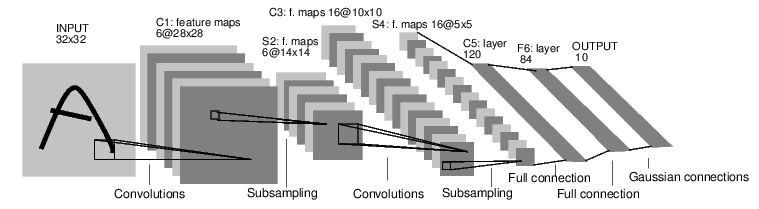
\includegraphics[scale=0.5]{figures/lenet5}
	\centering
	\caption{LeNet-5 Architecture \cite{lecun1998gradient}}
	\label{fig:lenet5}
\end{figure}


\subsection{Alex-Net}
Alex Net was proposed by Alex Krizhevsky, et al. \cite{krizhevsky2012imagenet} based on their winning on ILSVRC (ImageNet Large-Scale Visual Recognition Challenge) 2012. The architecture consists of eight layers: five convolutional and three fully-connected layers. The first convolutional layer is using a 11x11 filter size with a stride of 4. The other convolutional layer use 3x3 filter size. The subsampling layer that was used is max-pooling. An architecture of Alex-Net can be seen in figure \ref{fig:alexnet}. It was tested on ILSVRC 2012 dataset and achieves top 5 test error rate of 15.4\%.
\begin{figure}[h]
	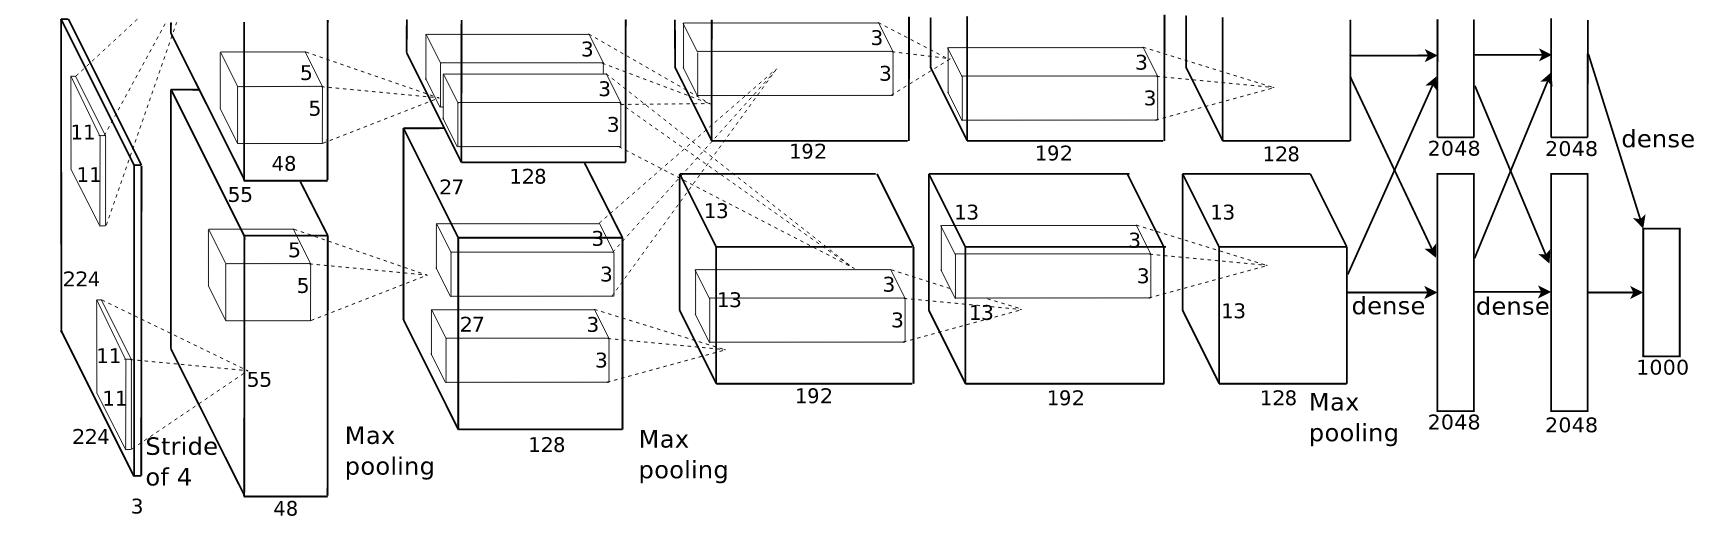
\includegraphics[scale=0.25]{figures/alexnet}
	\centering
	\caption{Alex Net Architecture \cite{krizhevsky2012imagenet}}
	\label{fig:alexnet}
\end{figure}
%\subsection{ZF-Net}
%ZF-Net was proposed by Zeiler and Fergus \cite{zeiler2014visualizing}. It was the winner of ILSVRC 2013. ZF-Net is a modification from Alex-Net. One of the differences between ZF-Net and Alex-Net is the filter size in the first layer, instead of using 11x11 with stride 4 like Alex-Net did, ZF-Net using 7x7 filter size with stride 2. The full architecture of ZF-Net can bee seen in figure \ref{fig:zf}. It was tested on the ILSVRC 2012 dataset and achieved 11.2\% error rate.

%\begin{figure}[h]
%	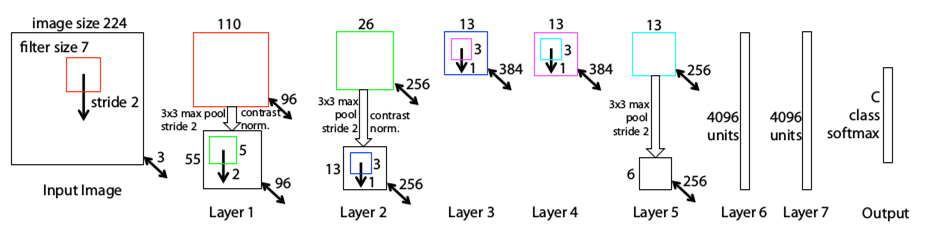
\includegraphics[scale=0.5]{figures/zfnet}
%	\centering
%	\caption{ZF Net Architecture \cite{zeiler2014visualizing}}
%	\label{fig:zf}
%\end{figure}


\subsection{VGG Net}
VGG Net was proposed by Karen Simonyan and Andrew Zisserman \cite{simonyan2014very} based on their winning on ILSVRC 2014. The architecture has 6 variations as shown in figure \ref{fig:vgg}. The key idea of this architecture is using a 3x3 filter size with a stride of 1 for every convolutional layer. In subsampling layer, VGG-Net uses 2x2 max pooling layer with stride size of 2. It was tested on ILSVRC-2012 dataset and can achieve a top-5 test error of 6.8\%.

\begin{figure}[h]
	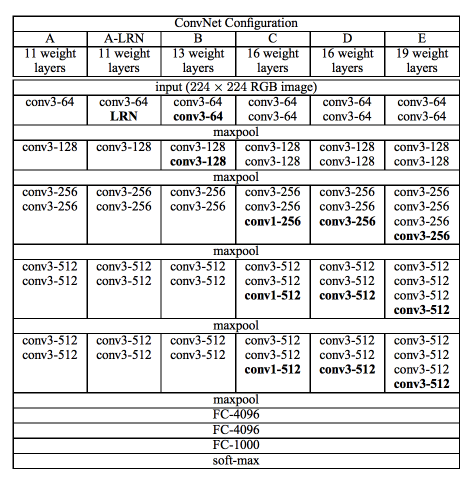
\includegraphics[scale=0.5]{figures/vggnet}
	\centering
	\caption{VGG Net Configuration \cite{simonyan2014very}}
	\label{fig:vgg}
\end{figure}


\subsection{ResNet}
In 2015, Microsoft proposed a very deep architecture called ResNet \cite{he2016deep}. It can go up to 1202 layers, but the best results for CIFAR-10 dataset is 6.43\% error rate by using 110 layers. The idea behind ResNet is stacking convolutional layer with 3x3 filter size until it reaches a very deep network. This initial version of ResNet also called ResNetV1. In 2016, ResNetV2 is introduced \cite{he2016identity} as improvement from ResNetV1.

%\subsection{Simple Net}

\section{Dataset}
Benchmarking the proposed deep learning architecture can be done by collecting some datasets to evaluate the architecture that was presented before. Here we presents some interesting image datasets.
\subsection{MNIST}
The MNIST Datasets (http://yann.lecun.com/exdb/mnist/) is a dataset of handwritten digits with 784 features (28x28 grayscale images). There are 10 classes, 60,000 training examples and 10,000 testing examples. An example of MNIST dataset can be seen in figure \ref{fig:mnist}.

We choose this dataset because it is heavily used as validation datasets for image recognition learning algorithm. Also it doesn't need preprocessing and formatting steps since the data is quite clean, thus we can focus on the learning implementation.

\begin{figure}[h]
	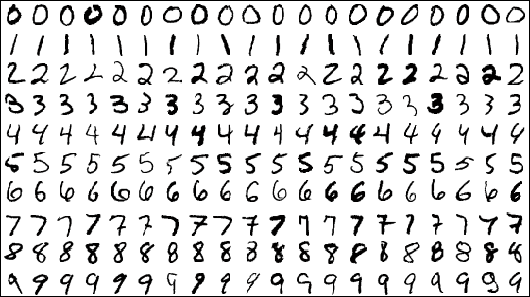
\includegraphics[scale=0.3]{figures/mnist}
	\centering
	\caption{An example of MNIST dataset}
	\label{fig:mnist}
\end{figure}

\subsection{Fashion-MNIST}
Fashion-MNIST \cite{xiao2017/online} is a dataset of Zalando's article images consisting of a training set of 60,000 examples and a test set of 10,000 examples. Each example is a 28x28 grayscale image, associated with a label from 10 classes. Zalando intends Fashion-MNIST to serve as a direct drop-in replacement for the original MNIST dataset for benchmarking machine learning algorithms. It shares the same image size and structure of training and testing splits.

Compared to MNIST, this datasets are quite new. Thus, unlike MNIST, these datasets are not heavily studied. We choose this datasets because of the similarities with MNIST datasets in terms of image size and representation. 
\begin{figure}[h]
	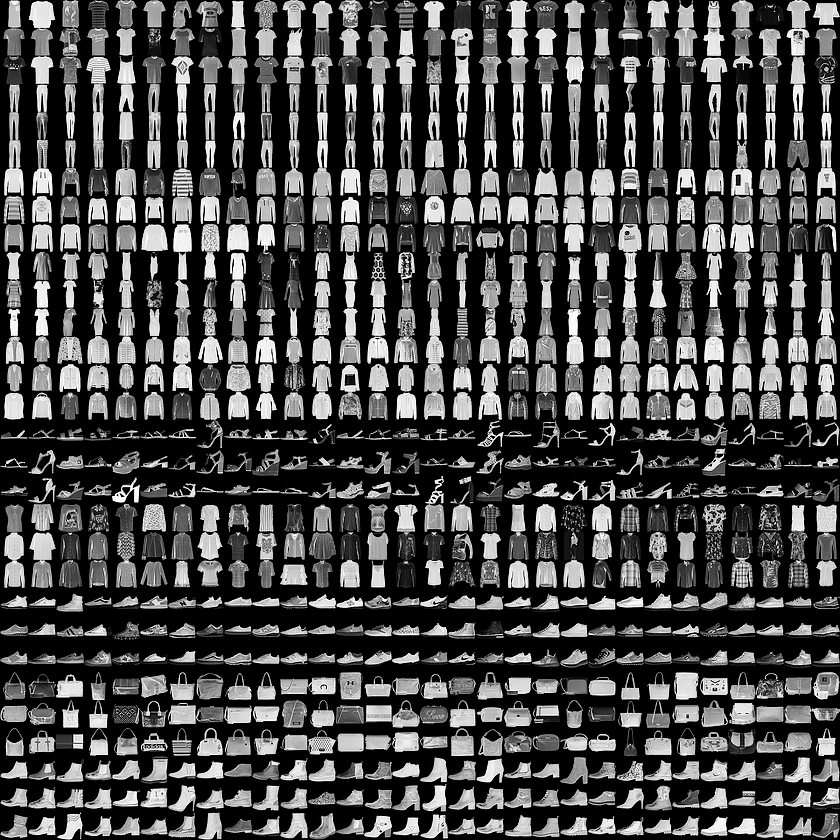
\includegraphics[scale=0.3]{figures/fashion-mnist}
	\centering
	\caption{Fashion-MNIST sprite. Each three rows in the sprite corresponds to a single class example. \cite{xiao2017/online}}
	\label{fig:fashionmnist}
\end{figure}

\subsection{CIFAR-10}
CIFAR-10 is a labeled subset of the 80 million tiny images dataset that were collected by Alex Krizhevsky, Vinod Nair, and Geoffrey Hinton \cite{krizhevsky2009learning}. It consists of 32x32 color images representing 10 classes of objects: airplane, automobile, bird, cat, deer, dog, frog, horse, ship, truck. An example of CIFAR-10 dataset can be seen in figure \ref{fig:cifar10}.

CIFAR-10 contains 6000 images per class. The original train-test split randomly divided these into 5000 train and 1000 test images per class.
The classes are completely mutually exclusive. For example, there is no overlap between automobiles and trucks. "Automobile" includes sedans, SUVs, things of that sort. "Truck" includes only big trucks. Neither includes pickup trucks.



\begin{figure}[h]
	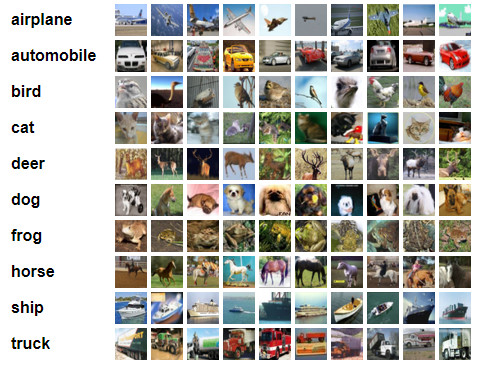
\includegraphics[scale=0.5]{figures/cifar10}
	\centering
	\caption{Example of CIFAR-10 dataset \cite{krizhevsky2009learning}}
	\label{fig:cifar10}
\end{figure}

%\subsection{CIFAR-100}
%CIFAR-100 \cite{krizhevsky2009learning} dataset is just like the CIFAR-10, except it has 100 classes containing 600 images each. There are 500 training images and 100 testing images per class. The 100 classes in the CIFAR-100 are grouped into 20 superclasses. Each image comes with a "fine" label (the class to which it belongs) and a "coarse" label (the superclass to which it belongs).

%\subsection{STL-10}
%STL-10 dataset \cite{coates2011analysis} is an image recognition dataset that were acquired from labeled examples on ImageNet. It is inspired by the CIFAR-10 dataset but with some modifications. In particular, each class has fewer labeled training examples than in CIFAR-10, but a very large set of unlabeled examples is provided to learn image models prior to supervised training. The primary challenge is to make use of the unlabeled data (which comes from a similar but different distribution from the labeled data) to build a useful prior. We also expect that the higher resolution of this dataset (96x96) will make it a challenging benchmark for developing more scalable unsupervised learning methods.

%There are 10 classes in this dataset: airplane, bird, car, cat, deer, dog, horse, monkey, ship, truck. Each images are colored 96x96 pixels.
%500 training images (10 pre-defined folds), 800 test images per class.
%100000 unlabeled images for unsupervised learning. These examples are extracted from a similar but broader distribution of images. For instance, it contains other types of animals (bears, rabbits, etc.) and vehicles (trains, buses, etc.) in addition to the ones in the labeled set.


%\begin{figure}[h]
%	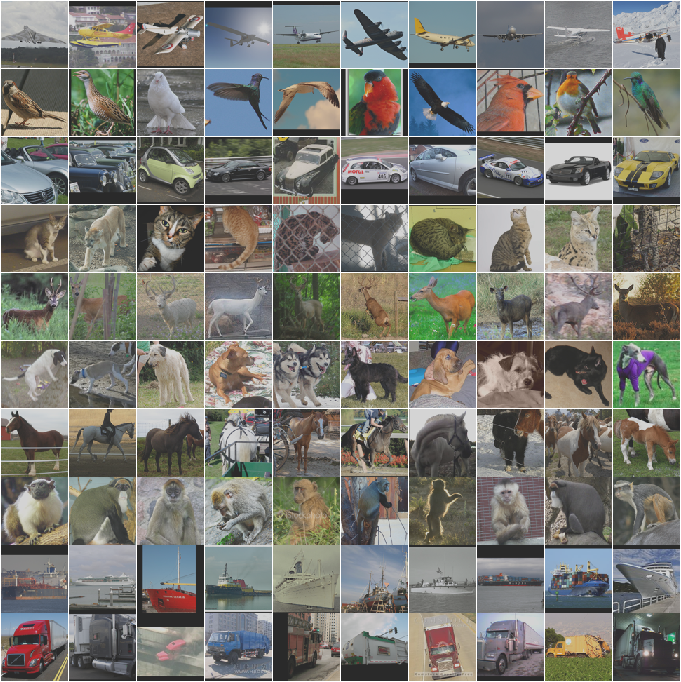
\includegraphics[scale=0.3]{figures/stl}
%	\centering
%	\caption{Examples of STL-10 datasets \cite{coates2011analysis}}
%	\label{fig:svhn}
%\end{figure}

\subsection{SVHN}
The Street View House Numbers (SVHN) Dataset \cite{netzer2011reading} is a dataset obtained from house numbers in Google Street View images. It is similar to MNIST (e.g., the images are of small cropped digits), but incorporates an order of magnitude more labeled data (over 600,000 digit images) and comes from a significantly harder, unsolved, real world problem (recognizing digits and numbers in natural scene images).

There are 10 classes, 73257 digits for training, 26032 digits for testing, and 531131 additional, somewhat less difficult samples, to use as extra training data. There are two formats of this datasets. The one that we are consider is the second format which is an MNIST-like dataset with 32-by-32 images centered around a single character (many of the images do contain some distractors at the sides).

\begin{figure}[h]
	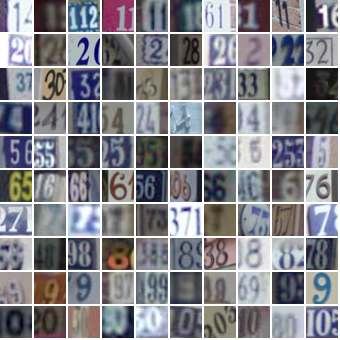
\includegraphics[scale=0.5]{figures/svhn}
	\centering
	\caption{Examples of SVHN datasets \cite{netzer2011reading}}
	\label{fig:svhn}
\end{figure}



%\clearemptydoublepage

\chapter{Experiment}\label{chapter:experiment}
%experiment
\section{Experiment Setup}
All of the experiment is executed on portable computer with specification as follows:
\begin{center}
	\begin{tabular}{| c| c| }
		Processor & Intel® Core™ i7 6700HQ Processor\\ 
		RAM & 8.0 GB \\  
		GPU & NVIDIA® GeForce® GTX 960M \\
		VRAM & 2.0 GB     
	\end{tabular}
\end{center}

For training process, we use Keras with TensorFlow as backend library. Python version that was used is 3.6. For every experiment, we limit it to 10 epochs since the amount to train 1 epoch is quite high.

\subsection{Architecture Implementation}
Since we are testing on a less powerful machine, we have to adjust the implementation of the architecture as follows \ref{code:lenet}
\subsubsection{LeNet}
We are not making any adjustment on implementing LeNet from its original version since the network itself is quite simple and straightforward. 
\ref{code:lenet}
\subsubsection{VGG-Net}

\subsubsection{ResNet V1}

\subsubsection{ResNet V2}
Implementing ResNet V2 is the same as ResNetV1. We just need to change the parameter of n=2 (so that the depth is equal to 20) and version=2.
\subsubsection{AlexNet/SqueezeNet}
Initially we plan to implement AlexNet. But, when we try to implement it on the current machine we failed to implement it because of hardware restriction. Then, we discover SqueezeNet \cite{SqueezeNet}.

\subsection{Dataset Preprocessing}
MNIST, Fashion MNIST and CIFAR-10 dataset are available directly from {\tt{keras.datasets}} package. The code to load these 3 datasets can be seen on Appendix \ref{code:mnist}, \ref{code:fashionmnist} and \ref{code:cifar10} respectively. As we can see from these codes, the only pre-processing steps applied for these 3 datasets are reshaping input to (28,28,1) (for MNIST and Fashion-MNIST) and converting classes from numerical type to categorical type.





\chapter{Results and Discussion}\label{chapter:analysis}
In this Chapter we report the results of the training and validation of the neural networks described in the experimental approach. Then, we discuss the results in terms of the research questions defined. Lastly, we assess the validity and limitations of our experimental procedure and results

\section{Experiment Result}
\begin{table}	
	\centering
	\begin{tabular}{ |c|c|c|c|c| } 
		\hline
		& MNIST & Fashion MNIST & CIFAR-10 & SVHN \\ 
		\hline
		LeNet-5	& 0.9834 & 0.8816 & 0.6561 & 0.809\\
		\hline 
		VGG-like & 0.9946 & 0.91 & 0.4075 & 0.067\\ 
		\hline
		Resnet20v1 & 0.9246 & 0.592 & 0.7567 & 0.866\\ 
		\hline
		Resnet20v2 & 0.9222 & 0.8425 & 0.679 & 0.893\\
		\hline
		SqueezeNet & 0.9858 & 0.8813 & 0.555 & 0.775\\
		\hline
	\end{tabular}
	\label{tab:accuracy}
	\caption{Accuracy table}
\end{table}

\begin{table}
	\centering
	\begin{tabular}{ |c|c|c|c|c| } 
		\hline
		& MNIST & Fashion MNIST & CIFAR-10 & SVHN \\ 
		\hline
		LeNet-5	& 220s & 220s & 330s & 220s\\
		\hline 
		VGG-like & 4986s	& 4469s & 6816s & 6526s\\ 
		\hline
		Resnet20v1 & 7970s & 7909s	& 7204s & 9310s\\ 
		\hline
		Resnet20v2 & 13900s & 	13910s & 	12060s & 	15693s\\
		\hline
		SqueezeNet & 13800s & 	13907s & 	13630s & 	17550s\\
		\hline
	\end{tabular}
	%\caption{Execution time for each experiment.}
	\label{tab:times}
	\caption{Execution time table}
\end{table}
Table \ref{tab:accuracy} shows the result of the experiments in terms of accuracy. The execution times and number of parametes for each experiment is shown on \ref{tab:times} \ref{fig:params}.



\begin{figure}[h]
	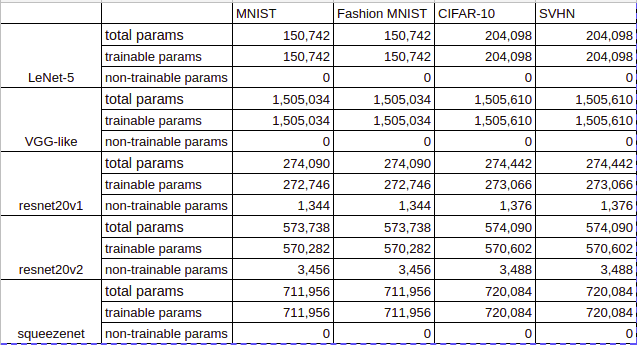
\includegraphics[scale=0.5]{figures/params}
	\centering
	\caption{Number of parameters for each experiment.}
	\label{fig:params}
\end{figure}

\section{Discussion}
In this Chapter, we reported the results of the experiments to answer the following research questions that was previously stated:

"How does the performance comparison of deep learning architecture model looks like for a given image classification dataset?"

\begin{enumerate}
	\item Which architecture that works bests for a given datasets?
	
	From table \ref{tab:accuracy}, we can see that VGG-like architecture performs the best on MNIST and Fashion MNIST dataset. ResNet20V1 and ResNet20V2 performs the best on CIFAR-10 and SVHN dataset respectively. In terms of memory usage and time consumption, it is proven that LeNet produces the simplest for all datasets.
	
	
	\item What kind of datasets characteristics that makes a deep learning architecture works well?
	
	From table \ref{tab:accuracy}, we can see that 
	\item Is there any architecture that generally works well for image classification?	
\end{enumerate}


 

\chapter{Conclusion}\label{chapter:conclusions}
Write your conclusions here.

%\clearemptydoublepage

%\chapter{Second Real Chapter}\label{chapter:second_real_chapter}
%In this Chapter we report the results of the training and validation of the neural networks described in the experimental approach. Then, we discuss the results in terms of the research questions defined. Lastly, we assess the validity and limitations of our experimental procedure and results

\section{Experiment Result}
\begin{table}	
	\centering
	\begin{tabular}{ |c|c|c|c|c| } 
		\hline
		& MNIST & Fashion MNIST & CIFAR-10 & SVHN \\ 
		\hline
		LeNet-5	& 0.9834 & 0.8816 & 0.6561 & 0.809\\
		\hline 
		VGG-like & 0.9946 & 0.91 & 0.4075 & 0.067\\ 
		\hline
		Resnet20v1 & 0.9246 & 0.592 & 0.7567 & 0.866\\ 
		\hline
		Resnet20v2 & 0.9222 & 0.8425 & 0.679 & 0.893\\
		\hline
		SqueezeNet & 0.9858 & 0.8813 & 0.555 & 0.775\\
		\hline
	\end{tabular}
	\label{tab:accuracy}
	\caption{Accuracy table}
\end{table}

\begin{table}
	\centering
	\begin{tabular}{ |c|c|c|c|c| } 
		\hline
		& MNIST & Fashion MNIST & CIFAR-10 & SVHN \\ 
		\hline
		LeNet-5	& 220s & 220s & 330s & 220s\\
		\hline 
		VGG-like & 4986s	& 4469s & 6816s & 6526s\\ 
		\hline
		Resnet20v1 & 7970s & 7909s	& 7204s & 9310s\\ 
		\hline
		Resnet20v2 & 13900s & 	13910s & 	12060s & 	15693s\\
		\hline
		SqueezeNet & 13800s & 	13907s & 	13630s & 	17550s\\
		\hline
	\end{tabular}
	%\caption{Execution time for each experiment.}
	\label{tab:times}
	\caption{Execution time table}
\end{table}
Table \ref{tab:accuracy} shows the result of the experiments in terms of accuracy. The execution times and number of parametes for each experiment is shown on \ref{tab:times} \ref{fig:params}.



\begin{figure}[h]
	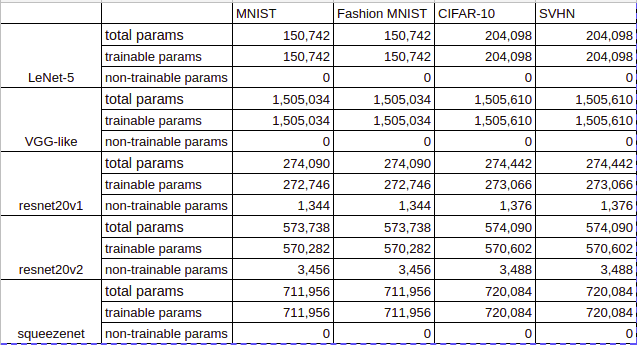
\includegraphics[scale=0.5]{figures/params}
	\centering
	\caption{Number of parameters for each experiment.}
	\label{fig:params}
\end{figure}

\section{Discussion}
In this Chapter, we reported the results of the experiments to answer the following research questions that was previously stated:

"How does the performance comparison of deep learning architecture model looks like for a given image classification dataset?"

\begin{enumerate}
	\item Which architecture that works bests for a given datasets?
	
	From table \ref{tab:accuracy}, we can see that VGG-like architecture performs the best on MNIST and Fashion MNIST dataset. ResNet20V1 and ResNet20V2 performs the best on CIFAR-10 and SVHN dataset respectively. In terms of memory usage and time consumption, it is proven that LeNet produces the simplest for all datasets.
	
	
	\item What kind of datasets characteristics that makes a deep learning architecture works well?
	
	From table \ref{tab:accuracy}, we can see that 
	\item Is there any architecture that generally works well for image classification?	
\end{enumerate}


 

%\clearemptydoublepage

%\chapter{Conclusions}\label{chapter:conclusions}
%Write your conclusions here.

%\clearemptydoublepage

%Choose a good bibliography style, plain would do often, but these might be nice too
%\bibliographystyle{these}
\bibliographystyle{plain}
\bibliography{references}

%\clearemptydoublepage

\appendix
\addcontentsline{toc}{chapter}{Appendix}
\chapter{My First Appendix}
In this file (appendices/main.tex) you can add appendix chapters, just as you did in the thesis.tex file for the `normal' chapters.
You can also choose to include everything in this single file, whatever you prefer.

\end{document}
